\documentclass[a4paper, 12pt]{article}%тип документа

%отступы
\usepackage[left=2cm,right=2cm,top=2cm,bottom=3cm,bindingoffset=0cm]{geometry}
\setlength{\parindent}{5ex}

%Русский язык
\usepackage[T2A]{fontenc} %кодировка
\usepackage[utf8]{inputenc} %кодировка исходного кода
\usepackage[english,russian]{babel} %локализация и переносы

%Вставка картинок
\usepackage{graphicx}
\graphicspath{{pictures/}}
\DeclareGraphicsExtensions{.pdf,.png,.jpg}

%Графики
\usepackage{pgfplots}
\pgfplotsset{compat=1.9}

%Математика
\usepackage{amsmath, amsfonts, amssymb, amsthm, mathtools}

%Таблицы
\usepackage{longtable} 
\usepackage{float}

%Римские цифры
\newcommand{\RomanNumeralCaps}[1]{\uppercase\expandafter{\romannumeral#1}}

\usepackage{multirow}


\begin{document}
	\begin{titlepage}
		\begin{center}
			\textsc{Федеральное государственное автономное образовательное учреждение высшего образования«Московский физико-технический институт (национальный исследовательский университет)»\\[5mm]
			}
			
			\vfill
			
			\textbf{Вопрос по выбору: \\[3mm]
			Измерение осмотического давления.
				\\[50mm]
			}
			
		\end{center}
		
		\hfill
		\begin{minipage}{.5\textwidth}
			Выполнил студент:\\[2mm]
			Сериков Василий Романович\\[2mm]
			группа: Б03-102\\[5mm]
			
		\end{minipage}
		\vfill
		\begin{center}
			Москва, 2022 г.
		\end{center}
		
	\end{titlepage}
	
	\newpage
	\textbf{Аннотация}\\
	
	
	\textbf{Цель работы: }\\
	
	1) Измерение осмотического давления при разной
	концентрации желтой кровяной соли; 2) Проверка закона Вант-Гоффа.\\
	
	
	\textbf{Теоретические сведения: } \\
	
	В работе изучаются свойства полупроницаемых перегородок, т. е. таких перегородок или мембран, сквозь
	которые молекулы одних веществ проходят, а молекулы других задерживаются.Так, многие перепонки и мембраны животного и растительного происхождения свободно пропускают молекулы воды, но не пропускают молекулы растворенных в ней соединений, обладающих большей молекулярной массой. Существуют также искусственные полупроницаемые перегородки, например, коллодиевые пленки, пленки из целлофана и др. Прохождение растворителя через полупроницаемую перегородку называется осмосом.
	Рассмотрим сосуд, разделенный на две части полупроницаемой перегородкой, по одну сторону которой находится вода,
	а по другую	— водный раствор вещества, молекулы
	которого не могут проходить сквозь перегородку (рис. 1).
	
		\begin{figure}[H]
	\center{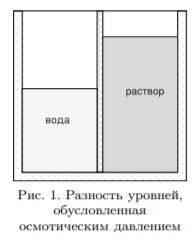
\includegraphics [scale=1]{photo_1.png}}
	\end{figure}
 Наполним обе части сосуда до одинакового уровня. Опыт показывает, что вода начинает переходить в ту
	часть сосуда, где содержится раствор. Этот переход продолжается
	до тех пор, пока между водой и раствором не	установится некоторая
	разность уровней, а следовательно,и разность давлений; она носит название осмотического давления раствора. Осмотическое давление оказывается довольно значительным даже при весьма малых	концентрациях растворенных веществ. Например, осмотическое давление сладкого чая относительно несладкого
	превышает 2 атм,а в клетках многих растений его величина составляет 5–20 атм, что обеспечивает поступление воды из почвы на большую высоту (например,
	к вершинам деревьев). Силу осмотического давления ощущают пловцы, открывая глаза в воде (особенно в пресной): внутриглазное давление повышается из-за поступления воды сквозь роговую оболочку.
	Осмотическое давление подчиняется формуле (закон Вант-Гоффа):
	\begin{equation}
 P_{\text{осм}} = n\cdot k_{\text{б}}\cdot T 
\end{equation}
	где	$n$ — число молекул растворенного вещества в единице объема,
	$ k_{\text{б}}$ — постоянная Больцмана,
	$T$ — абсолютная температура. Данная формула позволяет по известной величине
	$P_{\text{осм}}$ определить	концентрацию молекул растворенного вещества.\\

    \textbf{Экспериментальная установка: }\\
    
    Приборы, служащие для измерения осмотического давления, называют осмометрами. Прохождение растворителя через полупроницаемые перегородки происходит медленно, так что равновесие раствора и растворителя
    устанавливается не скоро. Для ускорения измерений над раствором создают избыточное давление воздуха. Если избыточное давление равно осмотическому, то переход растворителя через перегородку прекращается. Если же оно превышает осмотическое давление, то растворитель переходит через перегородку в обратном направлении. Таким образом, измерение осмотического давления сводится
    к измерению равновесного давления газа. Схема используемого в работе осмометра приведена на рис. 2. Раствор заливается в контейнер,
    который помещается в сосуд с растворителем. Контейнер представляет собой куб 1, закрытый с четырех сторон полупроницаемыми целлофановыми мембранами 3 (толщина
    мембран 0,2 мм). Мембраны зажимаются между стенками куба 1 и металлическими сетками 4. Между мембранами (пленками) и стенками куба вставлены резиновые уплотнения 7. Защитные сетки 4 предохраняют мембраны от раздувания наружу. Сосуд заполняется раствором через отверстие в дне куба, плотно закрываемое металлической гайкой 6 с резиновой прокладкой 24. Через крышку куба вставлен
    стеклянный капилляр 14 (внутренний диаметр 0,5 мм).
    В процессе осмоса объем раствора увеличивается, и уровень раствора движется по
    капилляру вверх. Скорость подъема уменьшается при избыточном давлении воздуха на верхнем конце капилляра; оно создается с помощью резиновой груши 23 со встроенным клапаном 25 и фиксируется краном 22. Давление измеряется манометром 21. Кран 22 также позволяет сбросить избыточное давление. На крышке куба 1 смонтировано устройство, состоящее из гофра 10, накидной гайки 11, винта 12
    и пружины 13, позволяющее менять объем внутреннего пространства в кубе. Это бывает необходимо, если в процессе опыта мембраны вытягиваются и уровень раствора в капилляре понижается. При закручивании винта 12 объем контейнера уменьшается и раствор вытесняется в капилляр. Таким образом
    уровень раствора можно установить в капилляре на удобной для наблюдения высоте.\\
    
    	\textbf{Методика измерений: }\\
    
    Для определения $P_{\text{осм}}$ измеряют изменение скорости $v$ движения
    уровня раствора в капилляре в зависимости от давления воздуха $P$
    и строят график зависимости $v(P)$. Чем больше разность давления
    $P - P_{\text{осм}}$, тем больше скорость $v$ движения уровня в капилляре. При
    $P \approx P_{\text{осм}}$ эта скорость равна нулю. Поэтому измерения следует проводить либо при $P \gg P_{\text{осм}}$, либо при $P \ll P_{\text{осм}}$. По графику легко определить значение $P$, при котором $v = 0$, т. е. осмотическое давление $P_{\text{осм}}$.
    В работе измеряется осмотическое давление водного раствора
    желтой кровяной соли $K_4Fe(CN)_6$, при нескольких значениях концентрации и проверяется справедливость закона Вант-Гоффа.
    Молекулы желтой кровяной соли при растворении диссоциируют;
    \begin{equation}
   		 K_4Fe(CN)_6 \rightarrow 4K^+ +[Fe(CN)_6]^{4-}
	\end{equation}
    Ионы $K^+$ свободно проникают через нашу перегородку и не создают
    осмотического давления.\\
    
    
    \textbf{Используемое оборудование: }\\
    
    Осмометр; секундомер; пипетка; мерный
    стаканчик; химический стакан.
    
    	\begin{figure}[H]
    	\center{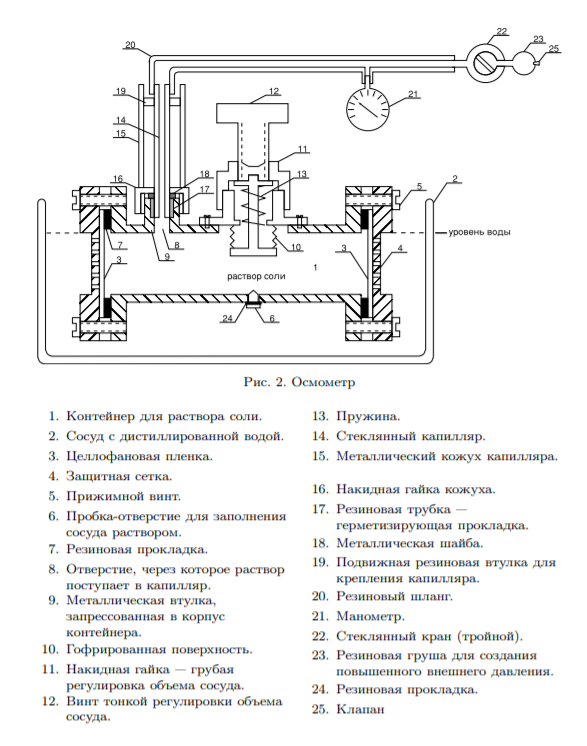
\includegraphics [scale=1.2]{photo_2.png}}
    \end{figure}
	
	
    \textbf{Результаты измерений и обработка данных: }
	
	\begin{enumerate}
		\item Запишем инструментальные погрешности.
		
		$\sigma_P = 1$ дел. (1 дел. = 245,17 Па), 
		$\sigma_t = 0,5$ с, 
		$\sigma_{\Delta l} = 1$ мм
		
		\item  Получим значения скорости ($v$ = [мм/с]) изменения уровня жидкости ($\Delta l $ = [мм]) в капилляре при различных давлениях для разных концентраций раствора (С = [г/л]). Полученные данные занесем в таблицы 1, 2, 3. (Различные знаки перед значением скорости означают различное направление движения столбика жидкости в капилляре)
	\newpage
		\begin{longtable} {|c|c|c|c|c|c|}
		\hline
		P, дел. & $ t $, с &   $ \Delta l$, мм  & $v$,  мм/с   & $\overline v $, мм/с & $\sigma_{\overline v}$, мм/с\\ \hline
		 \multirow{4}{*}{204}& 18,6 & 10 & 0,54 &  \multirow{4}{*}{0,54}    & \multirow{4}{*}{0,05}\\ \cline{2-4}
		 & 18,1 & 10 &    0,55         &               &\\ \cline{2-4}
		 & 18,7 & 10 &     0,53         &              & \\ \cline{2-4}
		 & 18,8 & 10 &    0,53           &             &\\ \hline
		 &&&&&\\ \hline
		 
		  \multirow{4}{*}{180}& 21,2 & 10 & 0,47 &  \multirow{4}{*}{0,48}    & \multirow{4}{*}{0,05}\\ \cline{2-4}
		 & 20,7 & 10 &    0,48         &               &\\ \cline{2-4}
		 & 21,0 & 10 &     0,48         &              & \\ \cline{2-4}
		 & 21,1 & 10 &    0,47           &             &\\ \hline
		 &&&&&\\ \hline
		 
		  \multirow{4}{*}{160}& 24,9 & 10 & 0,40 &  \multirow{4}{*}{0,41}    & \multirow{4}{*}{0,04}\\ \cline{2-4}
		 & 25,0 & 10 &    0,40         &               &\\ \cline{2-4}
		 & 24,5 & 10 &     0,41         &              & \\ \cline{2-4}
		 & 24,6 & 10 &    0,41           &             &\\ \hline
		 &&&&&\\ \hline
		 
		  \multirow{4}{*}{140}& 29,4 & 10 & 0,34 &  \multirow{4}{*}{0,34}    & \multirow{4}{*}{0,03}\\ \cline{2-4}
		 & 29,4 & 10 &    0,34         &               &\\ \cline{2-4}
		 & 28,2 & 10 &     0,35         &              & \\ \cline{2-4}
		 & 29,3 & 10 &    0,34           &             &\\ \hline
		 &&&&&\\ \hline
		 
		  \multirow{4}{*}{100}& 45,6 & 10 & 0,22 &  \multirow{4}{*}{0,22}    & \multirow{4}{*}{0,02}\\ \cline{2-4}
		 & 45,5 & 10 &    0,22         &               &\\ \cline{2-4}
		 & 43,6 & 10 &     0,23         &              & \\ \cline{2-4}
		 & 45,3 & 10 &    0,22           &             &\\ \hline
		 &&&&&\\ \hline
		 
		  \multirow{4}{*}{60}& 44,9 & 5 & 0,11 &  \multirow{4}{*}{0,11}    & \multirow{4}{*}{0,02}\\ \cline{2-4}
		 & 44,2 & 5 &    0,11         &               &\\ \cline{2-4}
		 & 44,7 & 5 &     0,11         &              & \\ \cline{2-4}
		 & 44,9 & 5 &    0,11           &             &\\ \hline
		 &&&&&\\ \hline
		 
		 \multirow{4}{*}{0}& 57,6 & 5 & - 0,09 &  \multirow{4}{*}{-0,06}    & \multirow{4}{*}{0,01}\\ \cline{2-4}
		 & 87,3 & 5 &    - 0,06         &               &\\ \cline{2-4}
		 &107,8 & 5 &     - 0,05         &              & \\ \cline{2-4}
		 & 116,2 & 5 &   - 0,04           &             &\\ \hline
		 &&&&&\\ \hline
		\caption{Результаты для $ C = 3 $ г/л  }
	\end{longtable}
	
	\newpage
	
	
	\begin{longtable} {|c|c|c|c|c|c|}
		\hline
		P, дел. & $ t $, с &   $ \Delta l$, мм  & $v$,  мм/с   & $\overline v $, мм/с & $\sigma_{\overline v}$, мм/с\\ \hline
		\multirow{4}{*}{200}& 10,4 & 10 & 0,96 &  \multirow{4}{*}{0,9}    & \multirow{4}{*}{0,1}\\ \cline{2-4}
		& 11,1 & 10 &    0,90         &               &\\ \cline{2-4}
		& 11,2 & 10 &     0,89         &              & \\ \cline{2-4}
		& 11,1 & 10 &    0,90           &             &\\ \hline
		&&&&&\\ \hline
		
		\multirow{4}{*}{180}& 12,9 & 10 & 0,78 &  \multirow{4}{*}{0,77}    & \multirow{4}{*}{0,08}\\ \cline{2-4}
		& 13,0 & 10 &    0,77         &               &\\ \cline{2-4}
		& 13,3 & 10 &     0,75         &              & \\ \cline{2-4}
		& 13,0 & 10 &    0,77           &             &\\ \hline
		&&&&&\\ \hline
		
		\multirow{4}{*}{160}& 15,2 & 10 & 0,66 &  \multirow{4}{*}{0,66}    & \multirow{4}{*}{0,07}\\ \cline{2-4}
		& 14,9 & 10 &    0,67         &               &\\ \cline{2-4}
		& 15,8 & 10 &     0,63         &              & \\ \cline{2-4}
		& 15,0 & 10 &    0,66           &             &\\ \hline
		&&&&&\\ \hline
		
		\multirow{4}{*}{140}& 17,9 & 10 & 0,56 &  \multirow{4}{*}{0,56}    & \multirow{4}{*}{0,06}\\ \cline{2-4}
		& 17,6 & 10 &    0,57         &               &\\ \cline{2-4}
		& 18,3 & 10 &     0,55         &              & \\ \cline{2-4}
		& 18,0 & 10 &    0,55           &             &\\ \hline
		&&&&&\\ \hline
		
		\multirow{4}{*}{100}& 26,7 & 10 & 0,37 &  \multirow{4}{*}{0,37}    & \multirow{4}{*}{0,04}\\ \cline{2-4}
		& 26,2 & 10 &    0,38         &               &\\ \cline{2-4}
		& 26,9 & 10 &     0,37         &              & \\ \cline{2-4}
		& 27,1 & 10 &    0,37           &             &\\ \hline
		&&&&&\\ \hline
		
		\multirow{4}{*}{60}& 26,5 & 5 & 0,19 &  \multirow{4}{*}{0,19}    & \multirow{4}{*}{0,04}\\ \cline{2-4}
		& 25,6 & 5 &    0,19         &               &\\ \cline{2-4}
		& 26,3 & 5 &     0,19         &              & \\ \cline{2-4}
		& 26,6 & 5 &    0,19           &             &\\ \hline
		&&&&&\\ \hline
		
		
		\multirow{4}{*}{0}& 128,9 & 3 & - 0,023 &  \multirow{4}{*}{- 0,021}    & \multirow{4}{*}{0,006}\\ \cline{2-4}
		& 133,8 & 3 &    - 0,022         &               &\\ \cline{2-4}
		& 139,7 & 3 &    - 0,022         &              & \\ \cline{2-4}
		& 149,5 & 3 &   - 0,020           &             &\\ \hline
		&&&&&\\ \hline
		\caption{Результаты для $ C = 1,5 $ г/л  }
	\end{longtable}
	
	
	\newpage
	
	
		\begin{longtable} {|c|c|c|c|c|c|}
		\hline
		P, дел. & $ t $, с &   $ \Delta l$, мм  & $v$,  мм/с   & $\overline v $, мм/с & $\sigma_{\overline v}$, мм/с\\ \hline
		\multirow{4}{*}{200}& 9,4 & 10 & 1,06 &  \multirow{4}{*}{1,1}    & \multirow{4}{*}{0,1}\\ \cline{2-4}
		& 8,9 & 10 &   1,12         &               &\\ \cline{2-4}
		& 9,4 & 10 &     1,06         &              & \\ \cline{2-4}
		& 9,5 & 10 &    1,05           &             &\\ \hline
		&&&&&\\ \hline
		
		\multirow{4}{*}{180}& 11,2 & 10 & 0,89 &  \multirow{4}{*}{0,9}    & \multirow{4}{*}{0,1}\\ \cline{2-4}
		& 10,5 & 10 &    0,95         &               &\\ \cline{2-4}
		& 10,7 & 10 &     0,93         &              & \\ \cline{2-4}
		& 10,8 & 10 &    0,93           &             &\\ \hline
		&&&&&\\ \hline
		
		\multirow{4}{*}{160}& 12,3 & 10 & 0,81 &  \multirow{4}{*}{0,79}    & \multirow{4}{*}{0,08}\\ \cline{2-4}
		& 12,7 & 10 &    0,79         &               &\\ \cline{2-4}
		& 12,6 & 10 &     0,79         &              & \\ \cline{2-4}
		& 13,2 & 10 &    0,76           &             &\\ \hline
		&&&&&\\ \hline
		
		\multirow{4}{*}{140}& 14,7 & 10 & 0,68 &  \multirow{4}{*}{0,68}    & \multirow{4}{*}{0,07}\\ \cline{2-4}
		& 14,5 & 10 &    0,69         &               &\\ \cline{2-4}
		& 14,4 & 10 &     0,69         &              & \\ \cline{2-4}
		& 15,2 & 10 &    0,67           &             &\\ \hline
		&&&&&\\ \hline
		
		\multirow{4}{*}{100}& 21,1 & 10 & 0,47 &  \multirow{4}{*}{0,46}    & \multirow{4}{*}{0,05}\\ \cline{2-4}
		& 22,0 & 10 &    0,45         &               &\\ \cline{2-4}
		& 21,9 & 10 &     0,46         &              & \\ \cline{2-4}
		& 22,5 & 10 &    0,44           &             &\\ \hline
		&&&&&\\ \hline
		
		\multirow{4}{*}{60}& 21,7 & 5 & 0,23 &  \multirow{4}{*}{0,24}    & \multirow{4}{*}{0,05}\\ \cline{2-4}
		& 21,2 & 5 &    0,24         &               &\\ \cline{2-4}
		& 20,6 & 5 &     0,24         &              & \\ \cline{2-4}
		& 20,6 & 5 &    0,24           &             &\\ \hline
		&&&&&\\ \hline
		
		
		\multirow{4}{*}{0}& 155,4 & 3 &- 0,019 &  \multirow{4}{*}{- 0,019}    & \multirow{4}{*}{0,006}\\ \cline{2-4}
		& 158,7 & 3 &    - 0,019         &               &\\ \cline{2-4}
		& 165,0 & 3 &    - 0,018         &              & \\ \cline{2-4}
		& 166,2 & 3 &   - 0,018           &             &\\ \hline
		&&&&&\\ \hline
		\caption{Результаты для $ C = 0,75 $ г/л  }
	\end{longtable}
	
	
	
	\item Подсчет погрешности проведем по формуле:
	
%	$$ \sigma_{\text{отд}} = \sqrt{\frac{1}{n - 1} \sum\limits_{i=1}^n (x_i - x_{\overline x})^2 } $$
	
	\begin{equation}
 \sigma_v = v \sqrt{\left(\frac{\sigma_t}{t}\right)^2 + \left(\frac{\sigma_{\Delta_l}}{\Delta_l}\right)^2 } 
\end{equation}

	% $$ \sigma_{\overline v} = \frac{\sigma_{v}}{\sqrt n}  $$
	
	\item Построим графики зависимости $ v(P) $. Точка пересечения полученных прямых с осью ординат покажет величину осмотического давления. Подсчет коэффициентов и погрешностей МНК проведем по формулам: 
	
\begin{equation}
	 k = \frac{\overline{vP} - \overline v  \overline P}{\overline{v^2} - \overline v ^2} 
\end{equation}
	
	\begin{equation}
		 b = \overline P - k \overline v 
	\end{equation}
	
	\begin{equation}
		 \sigma_{k_{\text{случ.}}} = \frac{1}{\sqrt n} \sqrt{\frac{\overline{P^2} - \overline P ^2}{\overline{v^2} - \overline v ^2} - k^2} 
	\end{equation}
		
	\begin{equation}
		\sigma_{k_{\text{сист.}}} = k \sqrt{\varepsilon_P^2 + \varepsilon_v^2}
	\end{equation}

	\begin{equation}
		\sigma_k = \sqrt{\sigma_{k_{\text{сист.}}}^2 + \sigma_{k_{\text{случ.}}}^2}
	\end{equation}

	\begin{equation}
		 \sigma_b = \sigma_k \sqrt{\overline{v^2} - \overline v ^2} 
	\end{equation}

	
	\begin{equation} 
		\sigma_{P_{\text{осм}}} = \sigma_b
	\end{equation}
	
	\item Тогда получим 
	
	
	\begin{figure}[H]
		\center{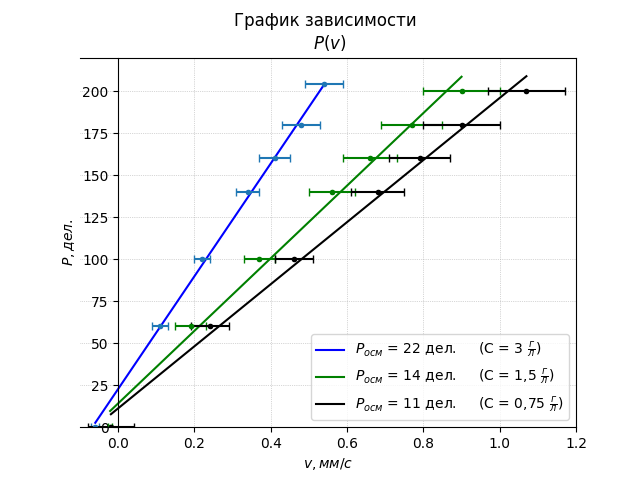
\includegraphics [scale=1]{P(v).png}}
	\end{figure}


	
	\begin{longtable}{|c|c|c|c|}
		\hline
	C, г/л	&  3  &  1,5 &  0,75 \\ \hline
	$P_{\text{осм}}$, кПа & 5,4$\pm 1,7$ & 3$\pm 1$& 2,7$\pm 0,8$ \\ \hline
	\caption{Значения осмотического давления.}
	\end{longtable}



\item Построим график зависимости осмотического давления от концентрации раствора 	$P_{\text{осм}}(C)$

\begin{figure}[H]
	\center{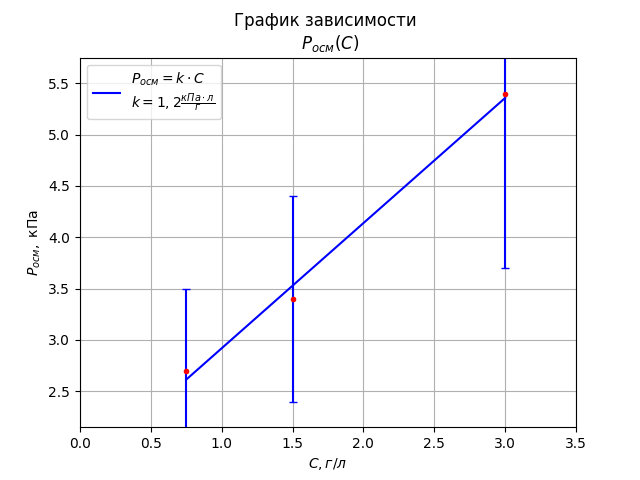
\includegraphics [scale=1]{P(C).png}}
\end{figure}

\item Тогда получим по МНК по формулам аналогичным (4)-(10) коэффициент наклона прямой $k = 1,2 \pm 0,4 \frac{\text{ кПа } \cdot \text{ л}}{\text{ г}}$

\item Из уравнения Вант-Гоффа имеем: 
	\begin{equation}
		 P_{\text{осм}} = \frac{\nu RT}{V} = C^{\text{мол}} RT 
	\end{equation}

Тогда в наших обозначениях, полученный коэффициент $k$:  
\begin{equation}
	k = \frac{RT}{\mu}
\end{equation}

Где $\mu = 368,35$ г/моль - молярная масса желтой кровяной соли, $T = 295$ К - температура в кабинете. 

\item Подсчитаем коэффициент $k$ по формуле (10), тогда получим $k = 6, 65 \frac{\text{ кПа } \cdot \text{ л}}{\text{ г}}$  
\end{enumerate}

\newpage
	\textbf{Обсуждение результатов: }\\
	
	
		В ходе данной работы мы получали значения скорости изменения уровня жидкости в капилляре. При различных давлениях можно было наблюдать прямой и обратный осмос, так как мы меняли внешнее давление. Точность полученных значений скорости не высока ($\varepsilon_v^{max} \approx 30\%$), так как измерения проводились на коротком отрезке капилляра, поэтому основной вклад в ошибку осмотического давления внесла погрешность измерения $\Delta l$.\\
		
		
		Построив график зависимости осмотического давления от концентрации по полученным давлениям, мы получили, что в нашем опыте линейная зависимость сохраняется. Однако закон Вант-Гоффа не выполняется, так как полученный в эксперименте коэффициент $k = \frac{RT}{\mu}$ отличается от полученного с помощью расчета по данной формуле в 5,5 раз. Можно предположить, что такое различие следует из особенностей осмометра: целлофановые пленки, выступающие в роли полупроводниковых мембран, используются на данной установке уже давно, и, возможно, имеют дефекты или имеет место не плотное соединение пленок со стенками осмометра, что влечет за собой выход раствора через образованные щели (так как давление $P_{\text{осм}}$ должно быть выше (следует из оценки полученного коэффициента $k$)).\\
		
	\textbf{Выводы: }\\
	
	
	У нас получилось измерить осмотическое давление при разной концентрации желтой кровяной соли. Мы проверили закон Вант-Гоффа, но подтвердить его не смогли, в силу технических особенностей установки.\\
	
	\textbf{Литература: }\\
	
1. Сивухин Д.В. Общий курс физики. Т. II. Термодинамика и молекулярная
физика, — М.: физматлит, 2005. Гл. XI, $\S$ 124.
	
	2. Гладун А.Д Лабораторный практикум по общей физике. Термодинамика и молекулярная физика, $\--$ М.: МФТИ, 2012. Гл. 2, работа 2.2.3 
	
\end{document}
	
	